\documentclass[border=2pt]{standalone}
\usepackage{tikz}
\begin{document}
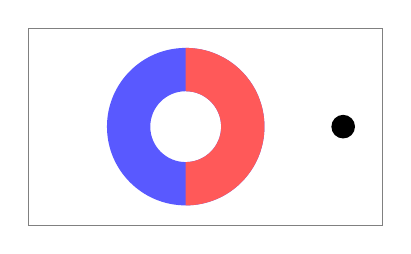
\begin{tikzpicture}
  \draw[gray] (-1,-1.25) rectangle (3.5,1.25);
  \begin{scope}[xshift=1cm,even odd rule]
    \clip (0,0) circle (1cm) (0,0) circle (.45cm);
    \fill[blue!65] (-2,-2) rectangle (2,2);
    \begin{scope}
      \path[clip] (0,-2) rectangle (2,2);
      \fill[red!65] (-2,-2) rectangle (2,2);
    \end{scope}
  \end{scope}
  \fill[black] (3,0) circle (.15cm);
\end{tikzpicture}
\end{document}
